%%=============================================================================
%% Case Study
%%=============================================================================

\chapter{Case study}%
\label{ch:casestudy}

\section{Introduction}%
\label{sec:introduction-casestudy}
This chapter will include the best practices and clean-up methods performed on the CI/CD pipeline at Wolters Kluwer and the metrics and results that were obtained from the clean-up. The chapter will include the CPU utilization, memory usage, build metrics, resource utilization, and system uptime of the CI/CD pipeline.

\section{Best Practices}%
\label{sec:best-practices}
The case study at Wolters Kluwer involved the implementation of best practices to improve the CI/CD pipeline. In following subsections the best practices are discussed.

\subsection{Remove build configuration with wrong Version Control System}%
\label{sub:remove-build-configuration-with-wrong-version-control-system}
The first best practice that was implemented was the removal of build configurations with the wrong version control system. This was done to ensure that the CI/CD pipeline was not cluttered with unnecessary build configurations. The removal of these build configurations helped to improve the efficiency and performance of the CI/CD pipeline.

\subsection{Detect build configurations with simultaneous running builds}%
\label{sub:detect-build-configurations-with-simultaneous-running-builds}
The second best practice that was implemented was the detection of build configurations with simultaneous running builds. This was done to identify build configurations that were running simultaneously and to ensure that the CI/CD pipeline was not overloaded. Simultaneous runnign builds can take a lot of resources and can slow down the CI/CD pipeline.

\subsection{Remove build configurations with no recent builds}%
\label{sub:remove-build-configurations-with-no-recent-builds}
Build configurations with no recent builds were archived or removed. This would help to reduce the clutter in the CI/CD pipeline and improve the performance of the pipeline.

\subsection{Remove artifacts of archived build configurations}%
\label{sub:remove-artifacts-of-archived-build-configurations}
Artifacts can take up a lot of space and those of archived build configurations are not needed anymore. This could free up a lot of space and improve the performance of the CI/CD pipeline.

\subsection{Automation of build agents}%
\label{sub:automation-of-build-agents}
By automating build agents, the CI/CD pipeline can be scaled up or down based on the demand. This would help to improve the scalability and usage of the CI/CD pipeline.

\subsection{Windows vs Linux}%
\label{sub:windows-vs-linux}
It was difficult to test this best practice. The reason behind this is that you need both operating systems. A build configuration that includes Powershell scripts can only be run on a Windows build agent. The same goes for Linux build agents. The best practice is to use Linux build agents as much as possible. This is because Linux build agents are more efficient and faster than Windows build agents.


\section{CPU Utilization}%
\label{sec:cpu-utilization}

The CPU utilization is shown in figure \ref{fig:cpu}. The clean up of the CI/CD environment hasn't reduced the CPU utilization clearly.

\begin{figure}[CPU]
    \centering
    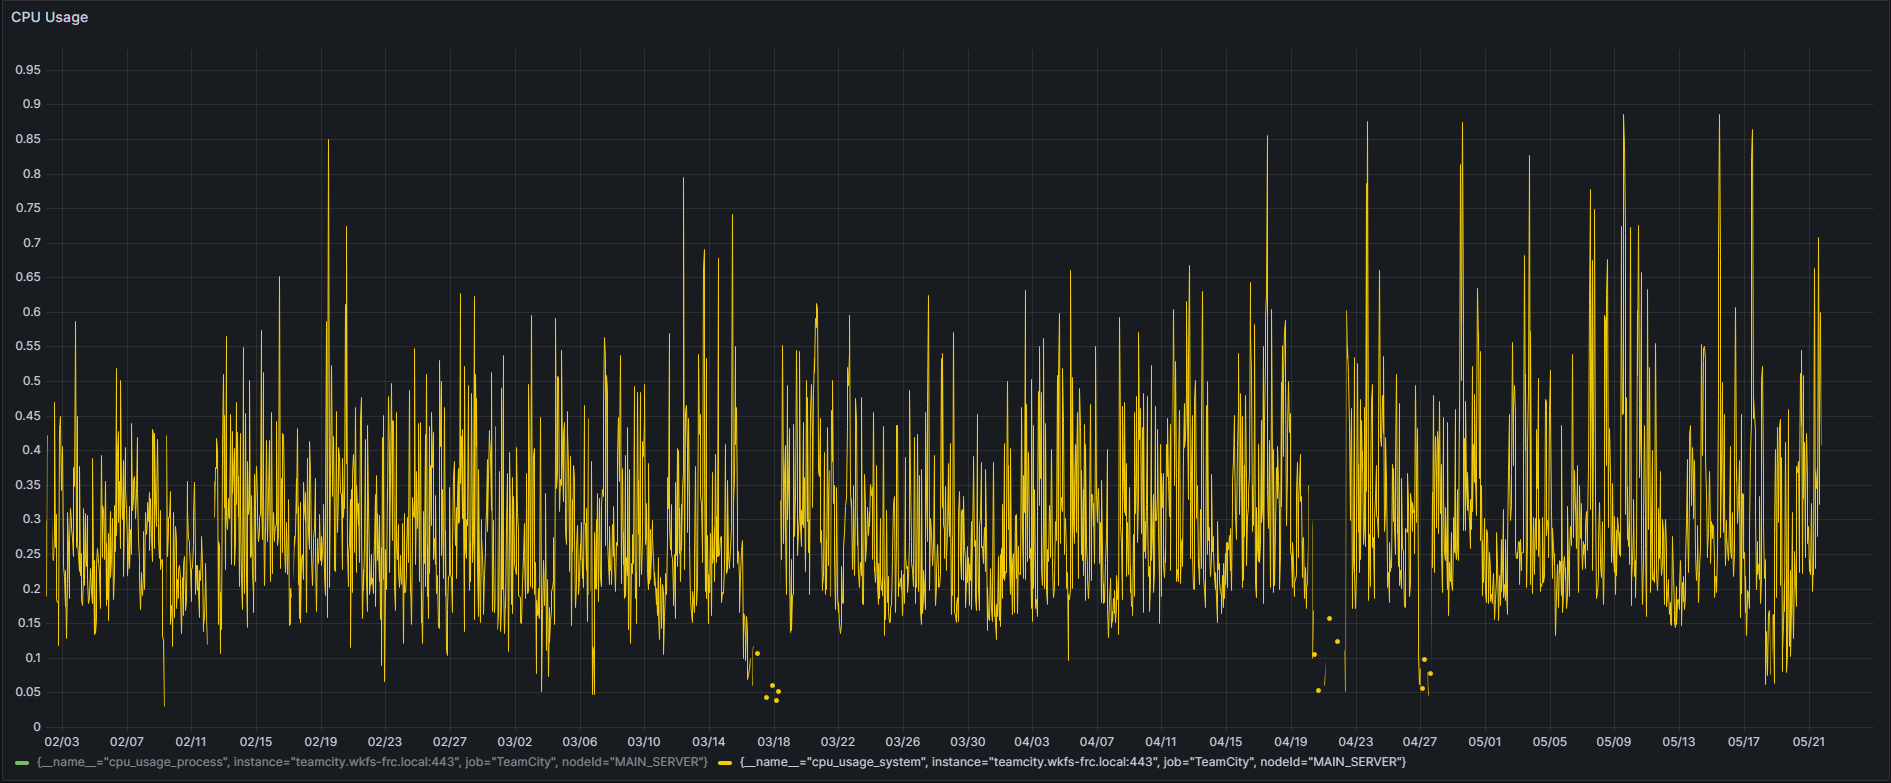
\includegraphics[width=\textwidth]{graphics/cpu.jpg}
    \caption{CPU Usage}
    \label{fig:cpu}
\end{figure}

